\chapter{Foundations of Digital Forensics}

\section{Intro and definitions}

\subsection{Digital and Electronic Evidence}

By the Scientific Working Group on Digital Evidence (\textbf{SWGDE}) a definition of, 
\textbf{digital evidence} is "any information of evidential value 
whether memorized or sent in a digital format". It's used by the \textbf{Council of Europe} \\

Another definition come from the \textbf{ Eoghan Casey - 2004} that define 
a d\textbf{igital evidence or electronic evidence} as "any probative informationstored 
or transmitted in digital form that a party to a court case may use at trial". It's more related to the 
juridical part. \\

A last definition of \textbf{Electronic evidence} is information generated, stored or transmitted
using electronic devices that may be relied upon in court, defined by the 
\textbf{Council of Europe - 2013}. \\

\begin{boxH}
    For the exam, the first dfinition is the more important
\end{boxH}

So. in general, way we can say that a digital/electronic evidence need to be:
\begin{itemize}
    \item \textbf{invisible} to the untrained eye
    \item Need to be \textbf{interpreted} by a specialist
    \item It may be \textbf{altered} or \textbf{destroyed} through normal use
    \item It can be \textbf{copied} without limits
\end{itemize} 

\subsubsection{Legal Requirements}
The main characteristics that a Digital/Electronic Evidence need to have to be accepted in a trial are:
\begin{itemize}
    \item \textbf{Admissability:} it need to be compliant with law and best practices. \\ 
        What can be seen is not what can be admissed in court (ex. if the italian police enter in a laptop, 
        can only "wiretapping", by enabling mic and camera, 
        and can't use other information like email or files in court )
    \item \textbf{Authenticity:} avoid any digital evidence tampering
    \item \textbf{Reliability and believability:} readily understandable for a judge. \\
        If a judge not understand the evidence can ignore it
    \item \textbf{Proportionality:} respect fundamental rights of parties affected by the measure
\end{itemize}

\subsubsection{Find a digital evidence}
A digital evicence can be hidden in different place and a criminal usully use some classical ways 
(not the cloud becasue the access is easy form a pocile force)
like hidden folder, usb, extrnal memory etc.. can be hidden everywhere 

\subsubsection{Categories}
Three main types of digital evidence
\begin{itemize}
    \item \textbf{Created by human}: digital data result of an action taken by an human
    \begin{itemize}
        \item \textit{Human to Human}: Like an email
        \item \textit{Human to PC}: like a word document
    \end{itemize}
    \item \textbf{Created indipendenlty by the computer}: data that are result of 
    the processing of data by an algorithm and without human intervention
    \item \textbf{Created by both human and the computer}: somethings like a spreadsheet where the data 
    are entered by the human, and the result is worked out by the computer
\end{itemize}

\newpage
\subsubsection{Julie Amero Case}

\begin{boxH}
    This case is not import for the exam
\end{boxH}

Julie Amero is a supply teacher at Kelly School in Norwich, Connecticut
who was found guilty of showing pornography to children under the age of 16
for some popup that appear during a lesson

\begin{figure}[h!]
    \centering
    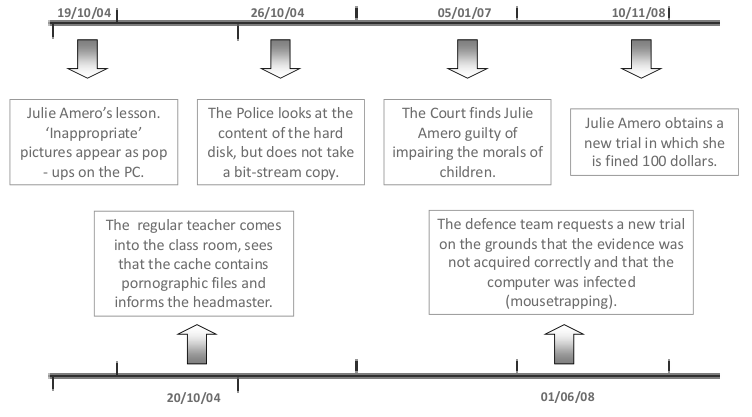
\includegraphics[width=1\textwidth]{img/amero_case.png}
    \caption{Timeline of the case}
    \label{fig:amero case}
 \end{figure}


\subsection{What is digital Forensics}

\textbf{Digital Forensics} is get hold of evidence without modifing the IT 
system in which that evidence is found, ensure that the 
evicence acuired in another medium is identical to the original and 
analyse data without modifyin it.

\subsection{The “Big Five” of Digital Forensics (Council of Europe)}

\begin{itemize}
    \item \textbf{Data Integrity:} No action taken \textit{should change electronic devices or media}, 
    which may subsequently be relied upon in court.
    \item \textbf{Chain of custody:} An \textit{audit trail} of all actions taken when handling electronic 
    evidence should be created and preserved
    \item \textbf{Specialist Support:} If investigations involving search and seizure of electronic 
    evidence it may be necessary to consult \textit{external specialists}. 
    \item \textbf{Appropriate Training:} First responders \textit{must be appropriately trained} to be able 
    to search for and seize electronic evidence if no experts are available at the scene
    \item \textbf{Legality:} The person and agency in charge of the case are responsible 
    for ensuring that \textit{the law and the above listed principles} are adhered to. 
\end{itemize}

\section{Digital Forensics Procedure}
Six phase of digital forensics procedure:

\subsection{Identify the Suspect}
There are 3 main phase for identify the suspect:

\begin{itemize}
    \item \textbf{Osint and Socmint:} Very usefull for collect information reguarding criminal 
    (even mafia ones), from social media, and other public sources.
    \item \textbf{Data Retension Directive in EU:} The investigator uses the Court 
    System to compel the ISP to reveal a physical location that 
    corresponds likely to the source of Network (IP Address)
    \item \textbf{Multiple User ID or multiple 
    Ips over time,  open Wi-Fi, Proxy, Botnet}: Under a warrant (depending from the Jurisdiction) 
    the location is searched and any computer or other device is seized
\end{itemize}

\subsubsection{Data Retension}
With the Directive 2006/24/EC, the EU member states are required to store data for 
a period of \textbf{6 to 24 months} (but can change from state to state). 
The data stored are gerally call detail records (CDR) of 
telephony and internet traffic and location data (IPDRs). \\
So evert single country and ISP have different data retention policy, and 
this can be a problem for the investigator, but from a privacy point of view a short time 
or null data retention is better.

\newpage

\paragraph{Transparency report:} Every year the ISP need to publish a transparency report 
where they show the number of request of data retention and the number of request that they 
have accepted.

\begin{figure}[h!]
    \centering
    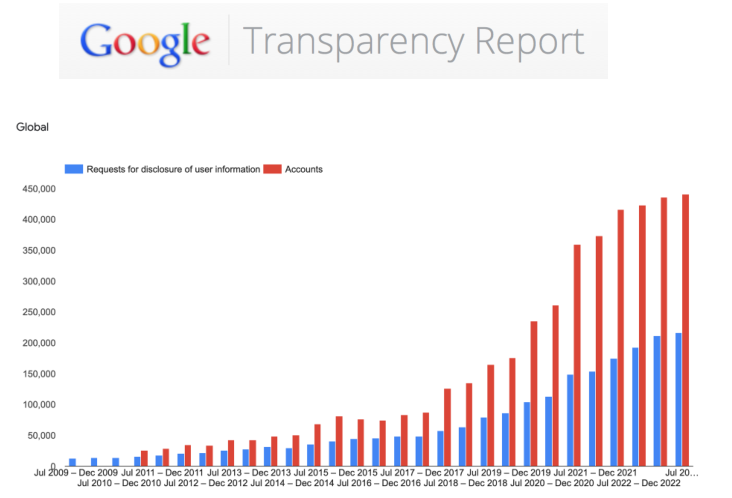
\includegraphics[width=0.6\textwidth]{img/transp_report.png}
    \caption{Timeline of Google transparency report}
    \label{fig:transparency report}
 \end{figure}

\subsubsection{Identify the suspect}
it's rigth use face recognision to identify a suspect? \\ 
For the moment if the situation is critical is possible utiliza A
live facial recognision. \\ 
AI act also regulate the use of facial recognision. % recuperare info dal testo del AI act

\subsection{Detecting and Seizing Digital Evidence}
The seize of digital evicences has torespet two foundamental rules: \textbf{bit-Stram Copy} and 
\textbf{Hash Function}. (definitions are alredy knowed)

\subsubsection{Where and how is the digital/electronic evidence hosted?}
The digital evicence can be in the suspected PC or in a third party server. \\
In the first case, we need to mange the encrition of the data, and it's possible get a Key Mandatory Law. \\
In the case of evicende in a server, is needed a collaborationfrom the ISP/Telco/Banck, and so need there is Jurisdiction problem. 

\subsubsection{The role of third paries during digital investigation}

A third party can give a lot of usefull information. \\
For example and \textbf{ISP} Could reveal from which place the email was sent, the \textbf{Mail Account Provider} could reveal from which places the email account was accessed and a \textbf{Credit Card Company} could reveal where the goods bought with a cloned credit card were delivered

\subsection{Validating Digital Evidence}
There is some tool that help to valdiate online digital evidence. \\
These kind of tool are usefull during OSINT bacasue they permit to collect data (like a story, a reel), that are not sure remain online, in a proper way for a court.


\subsection{Chain of Custody}

Digital storage media last less than analogue media and devices to read such media last even less. For example a LaserDisc last only 15 years, where there are books form thr 1086 (domesday book). So there at the moment, for trial, there are a lot of hard drive keeped in proprer way to avoid the data loss. It's a real mess.


\subsection{Analysis of Digital Evidence}

Start after the sieze of suspect's device, and need to be performed besided a precise chain of custody. \\ To perform the analysis are usually used some automatic tools, but in the recent time are used also some AI tools but only for post analysis and not for prediction policies (limitation imposed by the AI act) for example AI can not be used for kidnapping cases because the crime is in progress and not "finished".

\begin{itemize}
    \item \textbf{Text searches:} aimed at scanning files, directories and even entire file systems for specific text terms (generative AI can be used for summarizing and analyzing documents, but it's not very precise, plus alucination)
    
    \item \textbf{Image searches:} aimed at identifying image files in various formats, and at generating still frames of digitally stored video footage. Mainly analysis of child pornography that can be lead also to false positive (like a video of a mum and child in a bath)
    
    \item \textbf{Data recovery:} aimed at recovering all files stored on mass memory units, including deleted or damaged data. Destroy data can also be a crime (even if there are some backups), based on the intention of the crime (like delete file to hide evidence) 
    
    \item \textbf{Data discovery:} targeted at accessing hidden, encrypted or otherwise protected data
    
    \item \textbf{Data carving:} focused on reconstructing damaged files by retrieving portions of their content
    
    \item \textbf{Metadata recovery and identification:} this digital forensic tool is particularly useful for retracing the timeline of web accesses and file changes
\end{itemize}

Some other problem withthe use of \textbf{AI for prediction} of crime are: the bias of the AI and possible conseguences for privacy and \textbf{social control} by not very democratic government. 

\subsubsection{Two Italian issues}

\paragraph{Repeatable or Unrepeatable forensics analysis: }
\textbf{Repetable} when you can do a bit-stream copy of the data and also give one copy to the defence to do the same analysis, and more in general i can repeat analysis again and again (when i want). \\ In a \textbf{non-repetable} analysis, we need do live forensics activity and ofter occure with mobile phone, where there isn't the possibility to do a bit-stream copy of the data. In the live forensics i also need the presence of the attorney or the defender when i do the analysis to make it admissable in court.

\paragraph{Open Source or Closed Source:} %% recuperare da lezione
Open source can be more transparent 

\subsection{Presentation in Court}

The presentation of digital evidence findings is a \textbf{crucial stage} for prosecutors, judges, and lawyers (the evidence need to be presented in a way that the judge can understand it otherwire he can ignor it). The outcome of the trial relies not only on the results of the investigation but also on the \textbf{clarity and comprehensibility} of the report provided. \\

\textbf{Operational Recommendations:}
\begin{itemize}
    \item \textbf{Presence of an index:} The report should include a clear index for easy navigation through the document.
    \item \textbf{Glossary and Reference Notes:} If technical terms are used, a glossary and reference notes should be provided to ensure that all parties understand the terminology (judge and lawyers are not IT experts).
    \item \textbf{Timeline Table and Flow Charts:} A timeline table or flow charts should be included to visually represent the sequence of events and digital activities.
    \item \textbf{Presentation Slides with Photos:} Visual aids, such as presentation slides with photos, help in simplifying complex technical details.
    \item \textbf{Video Recording:} Where applicable, video recordings of the operations carried out during the investigation can provide further clarity.
\end{itemize}

\subsubsection{Presentation in Court of the Digital Evidence Findings: Murtha Case}

%% recuperare da lezione


\section{Privacy and Due Process Rights}

\subsection{Encryption}
Encryption can be used to hide the fact that encrypted messages are exchanged and used by criminals can lead to difficulties collecting the necessary evidence

\begin{figure}[!ht]
    \centering
    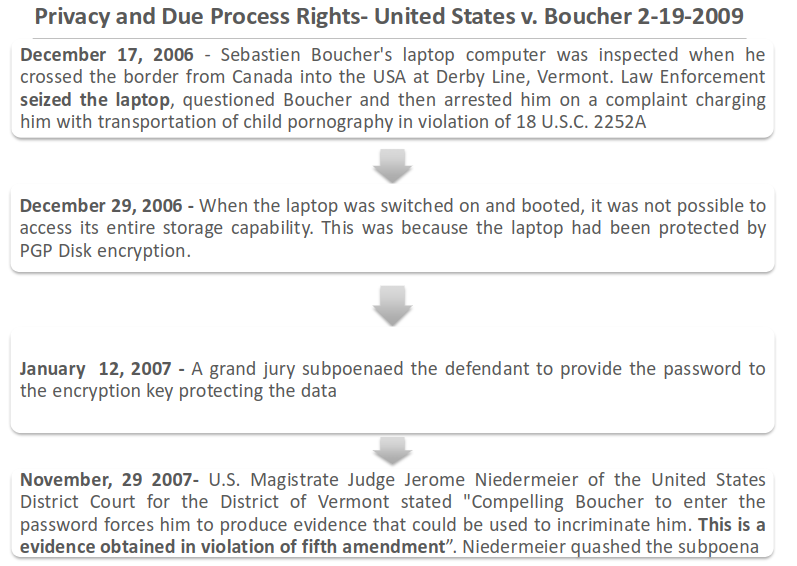
\includegraphics[width=0.5\textwidth]{img/enc_case.png}
    \caption{Case correlated with the use of encryption}
    \label{fig:encryption process}
\end{figure}

\newpage
\subsection{Case Law on Encryption}
Anther the previus case, some state are starting to create law about “Mandatory Key Disclosure" that force the suspect to give the key/password to decrypt the data. (some are Australia, Belgium France etc\dots) 

\subsection{Mandatory Key Disclosure Laws}
These case of legislative instrument doesn't work fow two main reason:
\begin{itemize}
    \item \textbf{technical reason:} An expert could always find a way yo hide a file
    \item \textbf{Possible violation of European Convention on Human Rights:} Article 6 Everyone charged with a criminal offence shall be presumed innocent until proved guilty according to law
\end{itemize} 

%% recuperare da lezione ---------

\subsection{Remote Forensics}

\begin{figure}[h!]
    \centering
    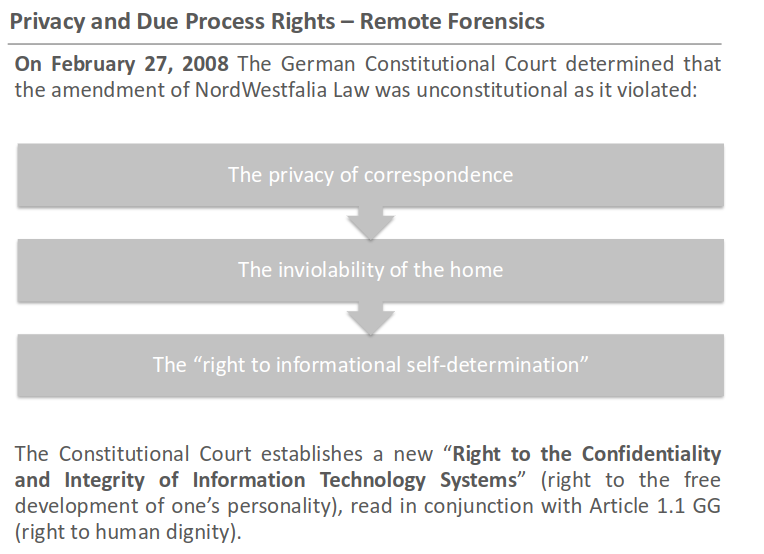
\includegraphics[width=0.4\textwidth]{img/remote_case.png}
    \caption{Case correlated to remote forensics}
    \label{fig:remote process}
\end{figure}

\subsection{Cloud Computing}

Cloud computing services face two key legal challenges: \textbf{Jurisdiction} and \textbf{Privacy}.

\paragraph{Jurisdiction}
The “\textbf{loss of location}” of digital evidence in the cloud introduces significant jurisdictional issues. In a cloud environment, the question arises: are the documents governed by the laws of the state in which they are physically located, the location of the company possessing them, or the laws of the state where the individual resides?

Over the last few years, various legal frameworks and approaches have been proposed to address this complex issue, but it remains an area of ongoing debate.

\paragraph{Privacy}
Cloud computing introduces several privacy concerns, including:
\begin{itemize}
    \item \textbf{Lack of Control:} Cloud clients may no longer maintain exclusive control over their data, limiting their ability to implement necessary technical and organizational measures to comply with \textbf{Data Protection Laws}.
    \item \textbf{Absence of Transparency:} Cloud providers may not provide sufficient information regarding how data is processed, leading to significant risks in terms of compliance with data protection regulations.
\end{itemize}


\subsubsection{Privacy} %% recuperare immagine da lezione




\subsubsection{Jurisdiction}  %% check, testo da GPT

In addressing the “loss of location” issue within the realm of cloud computing, we have four possible legal principles that can be applied:

\begin{itemize}
    \item \textbf{Territorial Principle:} The court in the jurisdiction where the data is physically located has authority. Jurisdiction is determined based on the geographical location of the data.
    
    \item \textbf{Nationality Principle:} The nationality of the perpetrator is used to establish criminal jurisdiction. The legal framework of the country of the individual committing the crime applies.
    
    \item \textbf{Flag Principle:} This principle applies to crimes committed on ships, aircraft, and spacecraft. They are subject to the jurisdiction of the country whose flag the vehicle flies under.
    
    \item \textbf{Power of Disposal Approach:} This approach focuses on who has control over the data. A regulation based on this would enable law enforcement to access a suspect's data in the cloud, regardless of its physical location, by considering the individual or entity with power over the data.
\end{itemize}

%% ------------------------------------